\documentclass[conference]{IEEEtran}
\usepackage[T1]{fontenc}
\usepackage{graphicx,amsmath,booktabs,url}
\usepackage[hidelinks]{hyperref}
\graphicspath{{figures/}}
\title{Does Blur Pooling Help a CIFAR-10 Classifier Trained on Shifted Images?}
\author{\IEEEauthorblockN{Haotian Si, Hongbo Yu, and Zifeng Zhou}
\IEEEauthorblockA{Rice University, Houston, Texas, USA\\ELEC 576 / COMP 576, Fall 2026}}
\begin{document}
\maketitle
\begin{abstract}
Moving a small image by one pixel can change its predicted class even when the object remains recognizable. We ask how much a fixed blur at both pooling stages contributes after a classifier has already learned from shifted images. We train twelve compact CIFAR-10 classifiers in a matched two-by-two experiment. Under one-pixel translations with reflected borders, blur reduces the mean prediction flip rate from 15.68\% to 10.04\% in the augmented models. Each of the three seeds improves. Mean clean and shifted accuracy change by $+0.04$ and $+0.11$ percentage points, meeting our prespecified accuracy limits. The one-pixel result persists with mean-filled borders and on a 9,000-image subset separated from the historical pilot. At four pixels with reflection, the mean flip-rate difference narrows to $-0.03$ points. The benefit depends on the scale of the displacement.
\end{abstract}

\section{Background and motivation}
A camera or cropper can move an object by one pixel between observations. For a 32-pixel-wide CIFAR-10 image this is a small displacement, yet it can change which activation wins a pooling window. Consider a bright vertical edge just inside the right half of a window. After a one-pixel translation, the largest response can fall in the neighboring window. A subsequent layer then sees that response at a different coarse-grid position. Repeating the operation deepens the dependence on the sampling grid. Figure~\ref{fig:translation} shows the corresponding change at the input. Large differences concentrate near edges even when a human recognizes the same object.

\begin{figure}[!ht]
\centering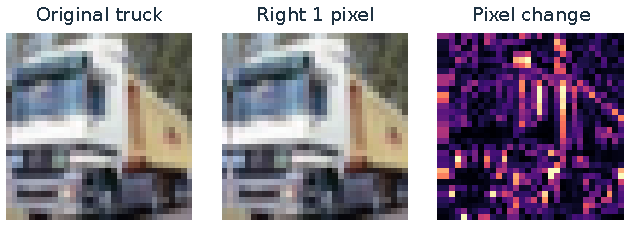
\includegraphics[width=\columnwidth]{translation.pdf}
\caption{An official training image and its one-pixel rightward translation. Reflection supplies the new left column. The last panel shows the mean absolute change across RGB channels, with brighter pixels indicating larger changes.}
\label{fig:translation}
\end{figure}

Translation augmentation gives a classifier examples of where an object might move. It places no architectural constraint on the response between examples. Azulay and Weiss observed sensitivity to small transformations even with convolution and augmentation~\cite{azulay2019}. Zhang evaluated filtering before subsampling on CIFAR-10 using circular shifts, which preserve pixels that cross the image boundary~\cite{zhang2019}. A shifted camera crop loses pixels at one edge. We study a compact classifier with reflected and mean-filled borders. After training with translations, how much more stability does blur provide, and at what accuracy cost?

We keep the response to a translation separate from the correctness of the response. A model can return the same wrong class five times. Conversely, a shift can correct a wrong answer. A decision based solely on consistency could reward a classifier that ignores informative detail. Our decision therefore combines the frequency of changes with two measures of label accuracy. We also change the rule for filling pixels exposed at the border. A reflected edge may itself provide a cue, especially in a small crop.

\subsection{A historical observation}
Zhou's Assignment 2 classifier used a 28-by-28 grayscale course subset and two conventional pooling layers~\cite{zhou}. Its regularized Setting C used reflected random crops and horizontal flips. We reconstructed the historical inference using the saved weights, the original normalization (mean 0.48215, standard deviation 0.23793), and the course test images in sorted directory order. The checkpoint predicted 631 of 1,000 original labels correctly. One-pixel shifts changed 816 of 4,000 predictions and produced 2,435 correct answers across the four views. These counts reproduce the proposal's 20.4\% flip rate, 63.1\% clean accuracy and rounded 60.9\% shifted accuracy.

The old training loop picked epoch 58 using the course test accuracy. Consequently the pilot provides evidence that the phenomenon occurs in this model family, but gives a biased starting point for estimating generalization. Reusing the weights would introduce another difference between the two studies. All formal classifiers start with new RGB-compatible weights, and all checkpoint choices use a dedicated clean validation set.

\section{Experimentation and model}
\subsection{Data, historical exposure, and splits}
The official CIFAR-10 Python archive contains 50,000 training and 10,000 test color images in ten classes~\cite{cifar,cifartech}. We verified the archive checksum, preserved the original sample order, and sampled 500 validation images per class from the official training partition with split seed 42. The remaining 4,500 per class form the training set. Channel means computed on those 45,000 images were (0.49184, 0.48254, 0.44682) on the unit interval. The population standard deviations were (0.24705, 0.24354, 0.26169). Every model used these same statistics.

Grayscale conversion and resizing invalidate exact file-hash comparisons between the course and official images. After freezing the experiment, we searched by content. For each official RGB image we formed grayscale candidates using three resampling rules and a center crop. We reduced each 28-by-28 candidate to 7-by-7 block means and retrieved the six nearest official images under each rule, searching both official partitions without using class labels. We then ranked the union by full-resolution root-mean-square pixel error under the best transform. We accepted a candidate at error at most three gray levels when the runner-up error was at least three levels and at least twice as large, with a separate rule for a unique exact match. We checked class agreement afterward.

Bicubic resizing gave the closest candidate for all 11,000 course images. The largest winning error was below 0.69 on the 0--255 scale. All 1,000 course test images matched distinct official test images. Of the 10,000 historical training images, 8,956 matched the formal training set uniquely and 1,043 matched validation uniquely. One training image had close alternatives and was retained as ambiguous. Its possible matches added no official test image to the exclusion set. We therefore also evaluate the models on the 9,000 test images remaining after exclusion. This is a sensitivity analysis based on identifiable exposure. The search cannot establish that all visually similar images represent distinct source scenes.

\subsection{Factorial comparison}
Both pooling sites in a given network use the same rule (Fig.~\ref{fig:design}). Conventional pooling takes a $2\times2$ maximum at stride two. MaxBlurPool first computes all overlapping $2\times2$ maxima at stride one. Each channel of that dense map is then filtered with
\[
 K=\tfrac{1}{16}
 \begin{bmatrix}1&2&1\\2&4&2\\1&2&1\end{bmatrix}.
\]
We retain centers at even row and column indices starting from zero. This sequence follows Zhang's downsampling design and the published implementation~\cite{zhang2019,adobe}. The blur is a registered buffer with no trainable entries. We reflect one position at each boundary of the dense map, excluding the edge sample itself. This internal feature-map padding stays fixed throughout the study.

\begin{figure}[!ht]
\centering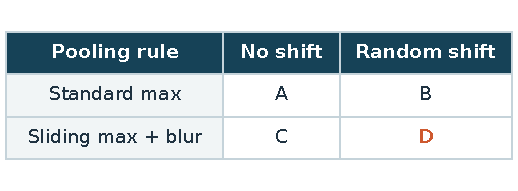
\includegraphics[width=\columnwidth]{design.pdf}
\caption{Four training conditions. The primary comparison moves from B to D within the random-shift column. C versus A estimates the blur effect for ordinary training images.}
\label{fig:design}
\end{figure}

The first convolution has six $5\times5$ kernels and two pixels of zero padding. Its output is $6\times32\times32$, followed by $6\times16\times16$ after pooling. A valid $5\times5$ convolution gives $16\times12\times12$ and the second pooling stage gives $16\times6\times6$. The dense stack maps 576 features through widths 120 and 84 to ten logits. Both convolutions and the first two dense layers use tanh. All four networks have 83,126 trainable parameters. The comparable shape at each site matters. Increasing the flattened width for just one variant would also change the capacity of the dense classifier.

Only B and D translate their training images. Horizontal and vertical offsets are independent uniform integers from $-2$ to $+2$, so the original location occurs with probability $1/25$. Positive offsets move image content right or down. Reflection fills newly exposed pixels without wrapping content from the opposite side. All four conditions omit horizontal flips. For evaluation we apply the same translation to every image in a given direction and keep labels fixed.

\begin{figure*}[!t]
\centering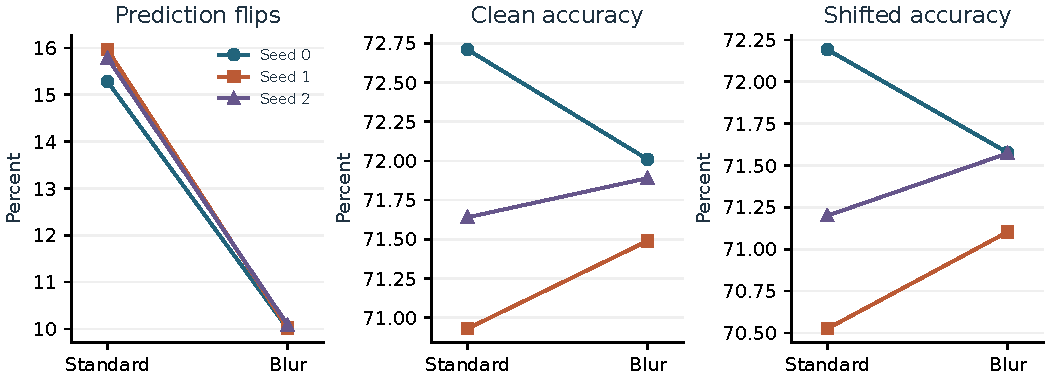
\includegraphics[width=.9\textwidth]{paired.pdf}
\caption{Primary outcomes on the 10,000 official test images. Each line connects the standard and blur models trained with identical initialization, sample order and shifts. The vertical scales differ across panels. Seed 0 trades some accuracy for stability. Seeds 1 and 2 gain on both accuracy measures.}
\label{fig:paired}
\end{figure*}

\subsection{Training, matching, and validation}
Training uses 60 epochs of cross-entropy minimization with SGD, momentum 0.9, weight decay 0.0005 and batches of 64. Each epoch includes its final short batch. The learning rate is 0.02 through epoch 25, 0.004 through epoch 40, and 0.0008 thereafter. The three seeds are 0, 1 and 2. For a given seed the four models begin with the same trainable parameter bytes. Every epoch uses an independent order stream shared across the four conditions. A separate stream supplies displacement pairs indexed by training sample, shared across B and D. We verified initialization, order and displacement hashes after the runs.

We chose the earliest epoch attaining the most correct predictions on 5,000 unshifted validation images. Neither test labels nor shifted validation scores enter this choice. Every run stores the selected weights, per-epoch losses and accuracies, and a restart state that includes the optimizer and learning-rate scheduler. We trained sequentially in FP32 on one RTX 5090 with TF32 disabled. A separate smoke run and one full-sized D timing epoch preceded the formal schedule. The timing epoch took 1.17 seconds including training and clean validation, excluding setup and checkpoint writes.

\subsection{Outcomes and decision rule}
For image $i$, let $c_i$ denote the clean predicted class, $y_i$ the true label, and $v_{id}$ the prediction for direction $d$. The reflected one-pixel flip rate is
\[
 F=\frac{1}{4N}\sum_{i=1}^{N}\sum_{d=1}^{4}\mathbf{1}[v_{id}\ne c_i].
\]
Shifted accuracy replaces the indicator by $\mathbf{1}[v_{id}=y_i]$. Clean accuracy uses $\mathbf{1}[c_i=y_i]$ once per image. For each matched seed we subtract the standard-pooling result from the blur result and multiply by 100 to obtain percentage points (pp). The primary contrast is D minus B. We call blur practically helpful only if every seed has a lower flip rate and the mean clean and shifted accuracies each fall by at most 1 pp. All secondary evaluations reuse the same selected checkpoints.

\section{Results}


\subsection{One-pixel shifts after augmentation}
All twelve runs completed 60 epochs. Table~\ref{tab:raw} gives the observed test values at the validation-selected epochs. For the augmented standard model, 15.68\% of reflected one-pixel comparisons changed the clean prediction on average. Blur reduced that fraction to 10.04\%, a decline of 5.64 pp or roughly 36\% of the standard model's flip rate. At 40,000 comparisons per checkpoint, the paired difference is about 2,256 fewer changes per seed. An image can change in more than one direction, so the number of affected images can differ from the number of changed comparisons.

\begin{table}[!ht]
\centering
\caption{Full-test results at the selected epoch. Flip, clean and shifted columns are percentages for the reflected one-pixel test.}
\label{tab:raw}
\begin{tabular}{ccrrrr}\toprule
Seed & Model & Epoch & Flip & Clean & Shifted\\\midrule
0&A&26&28.11&61.94&61.21\\
 &B&60&15.28&72.71&72.19\\
 &C&29&15.75&66.49&65.56\\
 &D&49&10.01&72.01&71.58\\\midrule
1&A&27&27.81&61.55&60.80\\
 &B&55&15.97&70.93&70.53\\
 &C&30&14.64&67.13&66.22\\
 &D&51&10.02&71.49&71.10\\\midrule
2&A&26&28.71&61.81&60.54\\
 &B&60&15.78&71.64&71.20\\
 &C&27&15.87&65.37&64.95\\
 &D&56&10.09&71.89&71.57\\\bottomrule
\end{tabular}
\end{table}

Figure~\ref{fig:paired} shows that the direction of the flip-rate effect is the same in every pair. Table~\ref{tab:paired} separates the accuracy effects. Seed 0 loses 0.70 pp clean accuracy, whereas the other two seeds gain. Across seeds, clean accuracy increases from 71.76\% to 71.80\% and shifted accuracy from 71.31\% to 71.42\%. Both mean differences are small compared with their between-seed variation. The prespecified criterion passes because it allows a small mean accuracy cost, and because the stronger consistency result holds for each seed. The accuracy results alone do not establish a general improvement.

\begin{table}[!ht]
\centering\caption{Matched differences in percentage points, computed before rounding. SD is the sample standard deviation across three training seeds.}
\label{tab:paired}
\begin{tabular}{lrrr}\toprule
D minus B & Flip & Clean & Shifted\\\midrule
Seed 0 & $-5.278$ & $-0.700$ & $-0.615$\\
Seed 1 & $-5.950$ & $+0.560$ & $+0.578$\\
Seed 2 & $-5.695$ & $+0.250$ & $+0.373$\\
Mean & $-5.641$ & $+0.037$ & $+0.112$\\
SD & 0.340 & 0.657 & 0.638\\\bottomrule
\end{tabular}
\end{table}

\subsection{What augmentation changes}
Without training translations, the mean flip rate changes from 28.21\% in A to 15.42\% in C. The three C-minus-A flip differences are $-12.36$, $-13.18$ and $-12.84$ pp. Clean and shifted accuracy increase by 4.56 and 4.73 pp on average. Thus blur contributes a larger absolute effect when training lacks translations. The difference between the paired mean effects is 7.15 pp. A substantial part of the stability that blur supplies alone is already present after translated-image training. The near equality of B and C flip rates is only part of the comparison. B achieves appreciably higher clean accuracy (71.76\% versus 66.33\%).

\subsection{Boundaries, distance, and historical exposure}
Figure~\ref{fig:border} shows how the incremental benefit changes with displacement. With one-pixel mean filling, the D-minus-B flip difference is $-5.87$ pp and shifted accuracy changes by $+0.18$ pp. The observed one-pixel effect thus persists when we change the input boundary. At two pixels the reflected difference is $-2.82$ pp, compared with $-3.12$ pp for mean filling. At four pixels these differences are only $-0.03$ and $-0.40$ pp. With four-pixel reflection, seed 0 even has a higher flip rate with blur ($+0.61$ pp). This distance exceeds the per-axis training range.

\begin{figure}[!ht]
\centering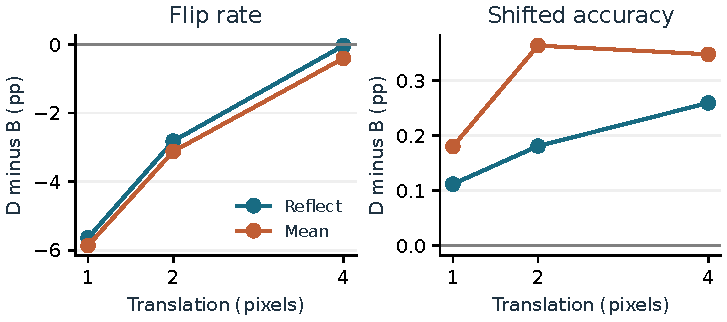
\includegraphics[width=\columnwidth]{borders.pdf}
\caption{Mean paired differences at three evaluation distances. Reflection and mean filling change only the input border. Network-internal blur always uses reflection. Negative flip differences and positive shifted-accuracy differences favor D.}
\label{fig:border}
\end{figure}

Absolute performance also depends on the border rule. At four pixels, D's mean shifted accuracy is 64.87\% with reflection and 62.06\% with mean filling. Filling with the training mean creates a uniform strip and removes edge detail. The direction of this accuracy difference describes this dataset and these weights. Individual images can react differently. The clean score is identical across these evaluations because the clean view never changes.

On the identifiable nonpilot subset the one-pixel reflected differences are $-5.66$ pp in flip rate, $+0.05$ pp in clean accuracy, and $+0.11$ pp in shifted accuracy. This close agreement with the full test makes it unlikely that the 1,000 historical test images alone drive the result. The subset shares 9,000 images with the primary analysis and uses the same trained classifiers. It checks sensitivity to exposure and supplies no additional independent training replicate.

\section{Discussion and conclusion}
As the proposal predicted, blur reduced one-pixel flips in all three augmented pairs. Accuracy varied in direction across seeds, and the four-pixel results limit how far the stability finding extends. Filtering a dense maximum map blends nearby responses before choosing a sampling phase. That mechanism is consistent with the largest reduction occurring at one pixel, where a phase change can switch which local evidence is retained. We did not measure internal frequency spectra or manipulate filter phase separately. The contrast estimates the effect of the entire pooling replacement, which also changes the effective receptive field.

Two stride-two stages give a cumulative sampling stride of four. A four-pixel translation can align interior features with the same downsampling phase, while moving the feature map relative to the dense classifier and replacing pixels at the edge. This offers one explanation for the shrinking incremental benefit at four pixels. Distance, phase, lost image content and departure from the training range vary together here. A follow-up could preserve visible content in a larger canvas and vary phase independently before drawing a mechanistic conclusion.

\begin{figure}[!ht]
\centering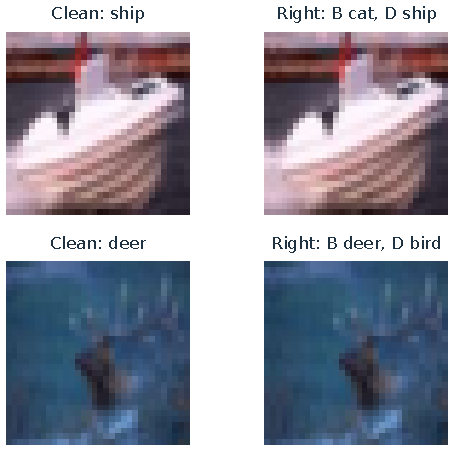
\includegraphics[width=.85\columnwidth]{examples.pdf}
\caption{Seed 0, one pixel right. Both models classify each clean image correctly. On test ID 108, B changes ship to cat and D retains ship. On ID 22, D changes deer to bird while B retains deer. Rows use the first qualifying test ID for each specified outcome.}
\label{fig:examples}
\end{figure}

Figure~\ref{fig:examples} illustrates why aggregate and individual claims differ. Blur preserves the correct ship prediction on one image and loses a correct deer prediction on another. A lower average flip rate gives no per-image guarantee. The conclusion also depends on the application. A system that prioritizes repeatability for one-pixel positioning errors may value a reduction of five or six flips per hundred views. A system exposed mainly to four-pixel crop changes receives much less evidence for the same choice.

\subsection{Verification, difficulties, and scope}
We checked known translations on small matrices, the equality of mean filling before normalization and zero filling afterward, model shapes, the fixed filter, matched random streams, and clean-validation tie breaking. A small single-channel normalization test exposed a helper that assumed three output channels. Making the accumulator follow the input channel count corrected the test and preserved the official RGB statistics. An initial network download was interrupted. An on-disk official archive passed the published checksum and supplied the data. All formal runs finished. Independent CPU and GPU restart checks recovered the same final parameter values on this system. On a short GPU test, CUDA graph replay and ordinary forward/backward SGD also produced equal weights.

Only three training repetitions support each paired mean. The 40,000 translated views share images and model weights, so treating them as independent training trials would understate uncertainty. We report all seeds and avoid a significance claim. The study concerns a shallow tanh network, a specific binomial filter, fixed training shifts and two border rules. It leaves open the response to subpixel motion, other classifiers and naturally moving cameras. A replication with independently chosen seeds would help quantify variation in the small accuracy differences. A follow-up could compare filter widths at matched validation budgets to test whether the distance dependence changes.

For this classifier and training protocol, adding fixed blur after translation augmentation meets the proposal's practical criterion for reflected one-pixel shifts. It reduces changes in all three pairs at essentially unchanged mean accuracy. Its four-pixel results give little reason to expect a similar incremental advantage for larger displacements.

\section*{Code availability}
The \href{https://github.com/Zifeng-Zhou/COMP576-Final/tree/codex/blur-pooling-final}{\texttt{codex/blur-pooling-final}} branch holds the source, training histories and paired results. The repository is available at \url{https://github.com/Zifeng-Zhou/COMP576-Final}. Follow the \href{https://github.com/Zifeng-Zhou/COMP576-Final/blob/codex/blur-pooling-final/README.md}{README} to verify the data, train the four conditions and evaluate the selected checkpoints. We retain the course materials, model weights and per-image predictions locally. The repository includes their verification records.

\newpage
\section*{Group Members Roles}
\textit{Proposal plan (draft).} The proposal assigned the responsibilities below. Before final submission, the team will update this section to reflect the contributions each member confirms.

\textbf{Zifeng Zhou} was assigned to adapt the classifier, implement standard max pooling and blur pooling, and document the pilot experiment.

\textbf{Haotian Si (team captain)} was assigned to coordinate the project, lead the 12 matched training runs, manage the training logs and checkpoints, integrate the project materials, and handle final submission.

\textbf{Hongbo Yu} was assigned to verify the dataset splits, image translations and padding methods, evaluate the models, and analyze prediction flip rates and classification accuracy.

\textbf{All members} planned to verify the experiments together, prepare the poster, write the final report, and present the poster.

Zifeng Zhou authored the earlier Assignment 2 report and supplied the historical materials used here. Codex assisted with implementation, execution, analysis and preparation of this pre-presentation draft.
\bibliographystyle{IEEEtran}
\bibliography{references}
\end{document}
